\section{Аналитические раздел}

\subsection{Марковские случайные процессы}

Марковский процесс --- случайный процесс, обладающий следующим свойством:
для каждого момента времени  $t_{0}$ вероятность любого состояния  системы в будущем при t > $t_{0}$
зависит только от состояния системы в настоящем t = $t_{0}$ и не зависит от того, как процесс развивался в прошлом.

Вероятностью i-ого состояния называется вероятность $P_{i}(t)$ того,
что в момент времени t система будет находиться в состоянии $S_{i}$.
Для любого момента t сумма вероятностей всех состояний равна единице.

Для марковских процессов используются уравнения Колмогорова, составляющиеся по следующему правилу:
в левой части каждого уравнения стоит производная вероятности состояния, а правая часть содержит столько членов сколько стрелок связано с данным состоянием.
Если стрелка направлена из состояния, то соответствующий член имеет знак <<->>, в состояние -- <<+>>.
Каждый член равен произведению интенсивности данной стрелки и вероятности того состояния, из которого исходит стрелка.

То есть строится система уравнений, которые имеют вид:

\begin{equation}
	p_i'(t) = \sum\limits_{j=1}^{n} \lambda_{ji}p_j(t) - p_i(t)
	\sum\limits_{j=1}^{n} \lambda_{ij},
\end{equation}

$n$ --- число состояний в системе;

$\lambda_{ij}$ --- интенсивность перехода системы из $i$-ого состояния в $j$-ое.

Для определения предельных вероятностей состояний необходимо в уравнениях Колмогорова заменить их производные нулями и решить полученную систему линейных алгебраических уравнений.

Одно из уравнений данной системы заменяется условием нормировки:

\begin{equation}
	\sum\limits_{i=1}^{n} p_i(t) = 1.
\end{equation}

Время стабилизации вероятности состояний с некоторым малым шагом $\Delta t$, считается найденным, когда выполняется соотношение:

\begin{equation}
	|p_i(t) -  \lim_{t \rightarrow \infty} p_i(t)| < \varepsilon,
\end{equation}

где $\varepsilon$ -- точность.

\section{Результаты работы}

На рисунке \ref{fig:r2} представлен результат работы программы c 3 состояними.

\begin{figure}[ht!]
	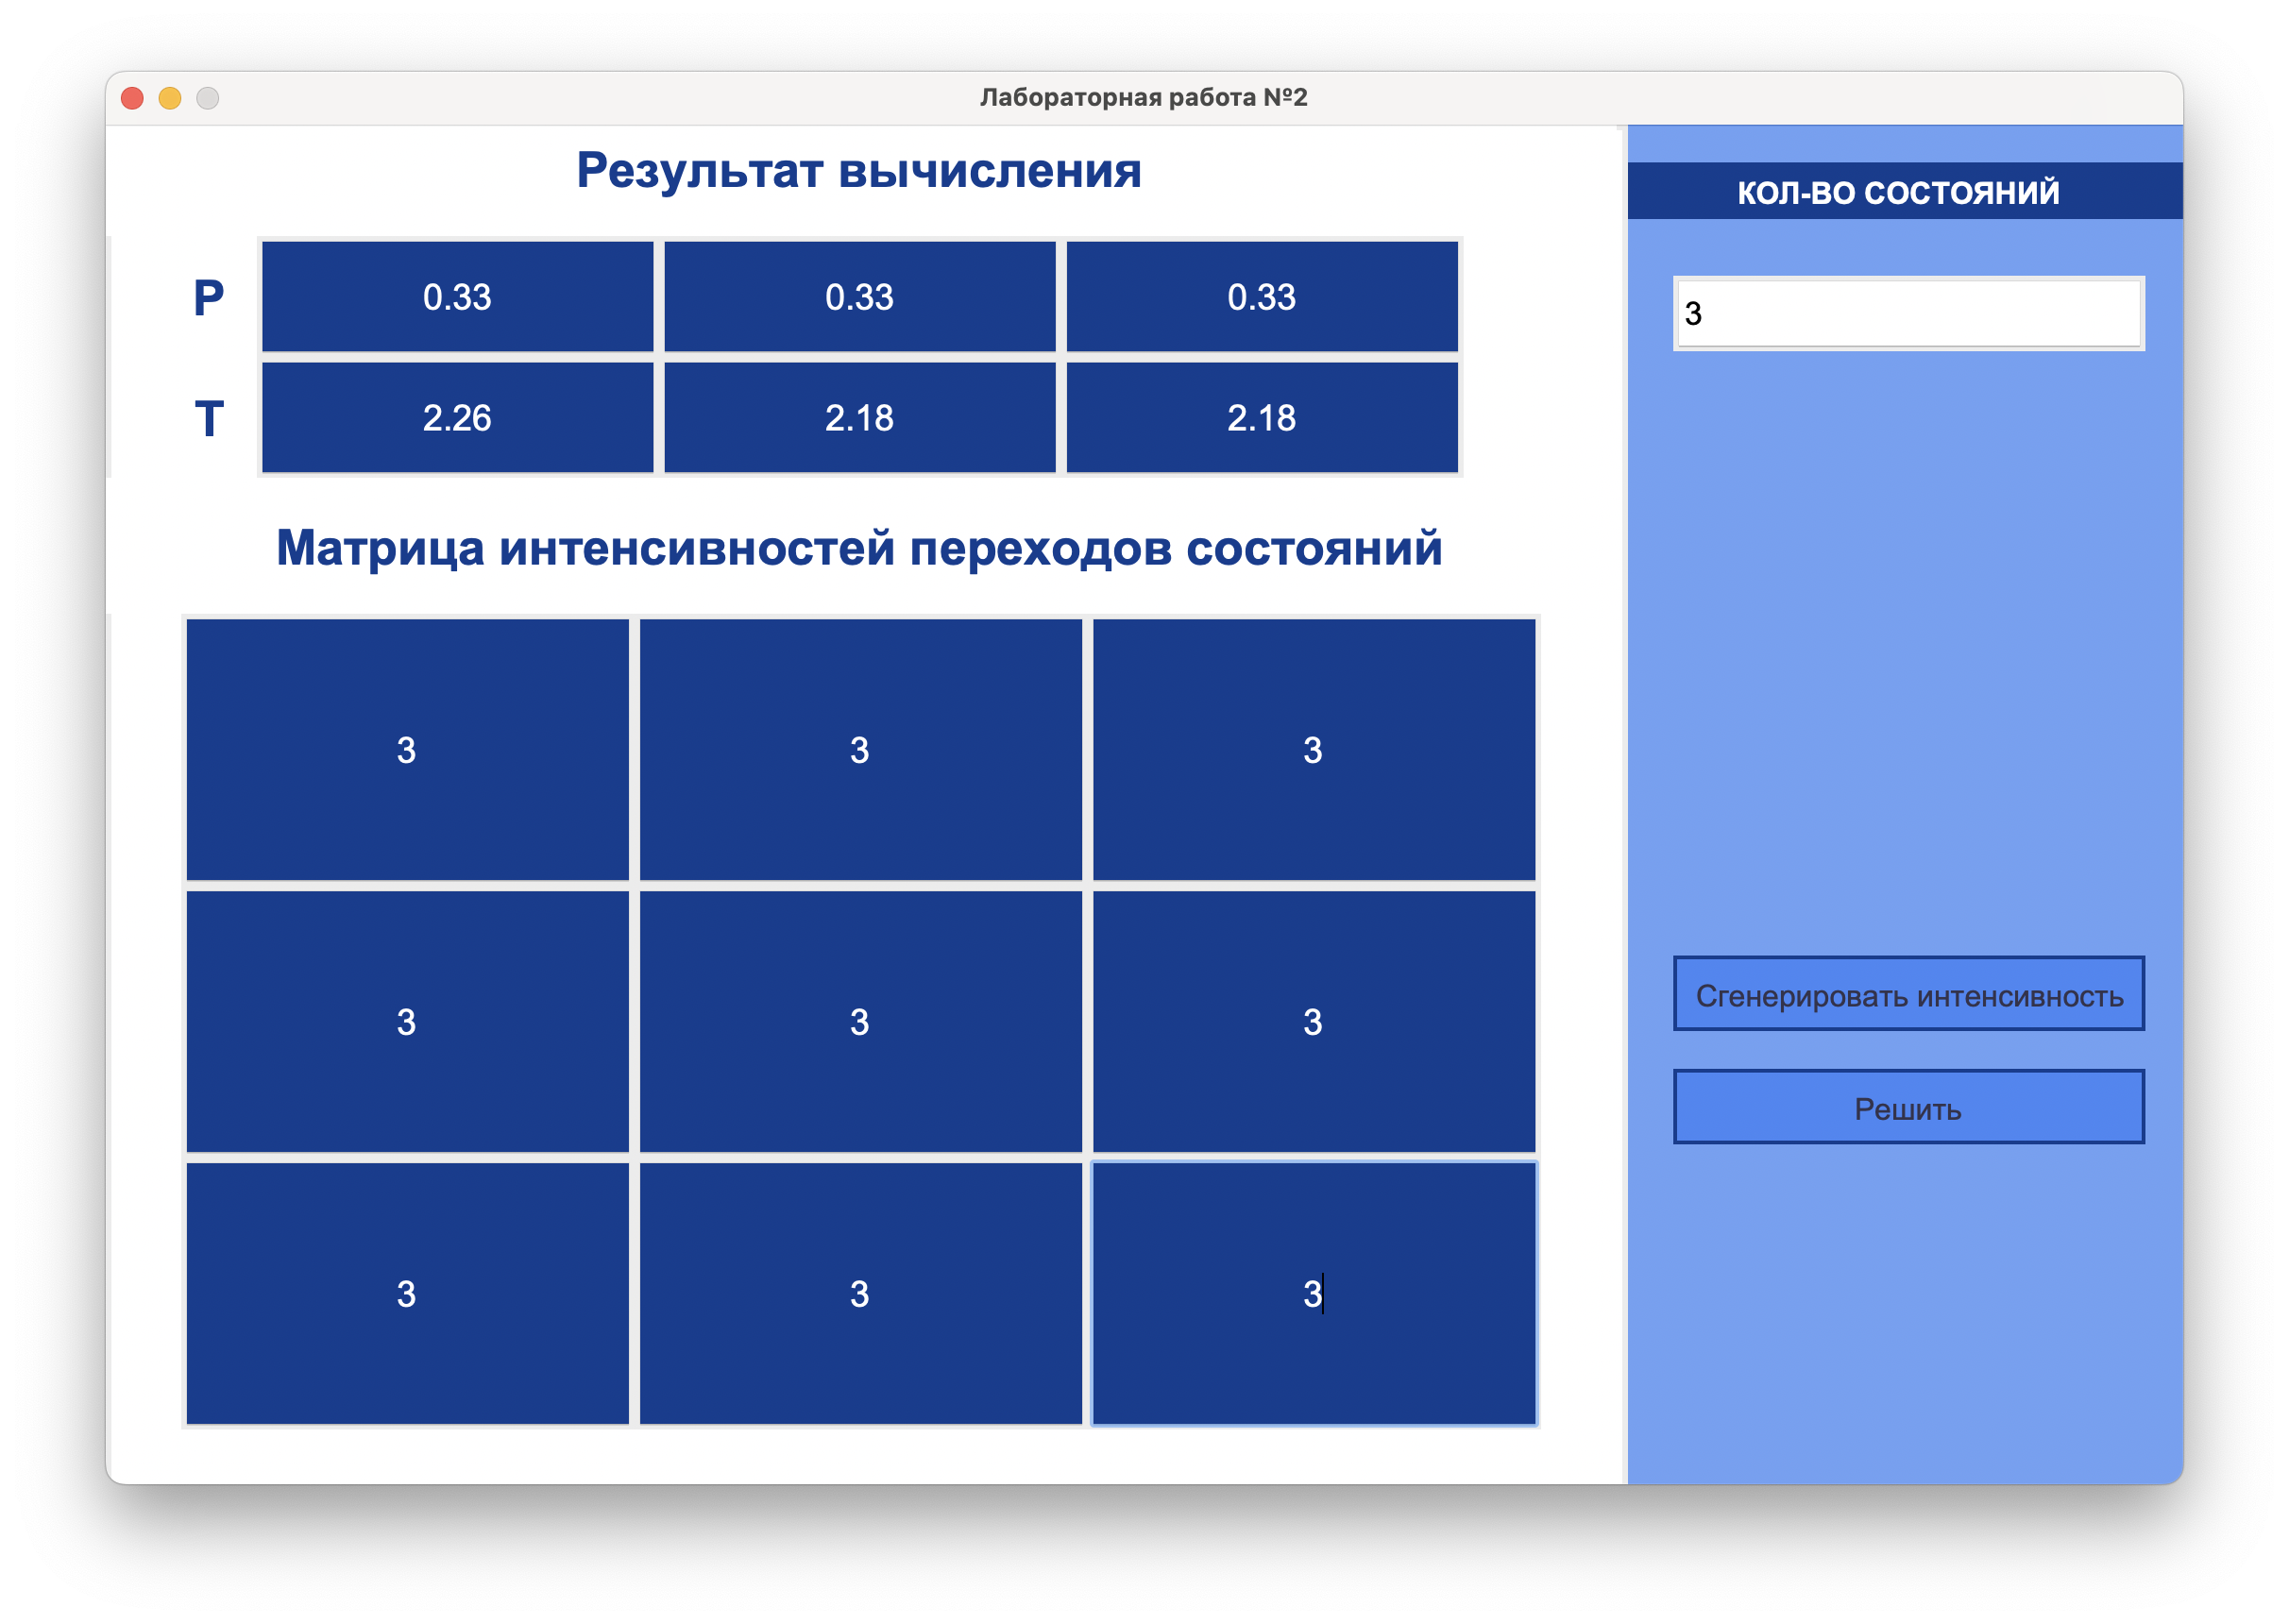
\includegraphics[width=0.75\linewidth]{assets/images/3_new.png}
	\caption{Результат работы программы с 3 состояними}
	\label{fig:r2}
\end{figure}